% ===========================================================================
% Introduction à l'Intelligence Artificielle
% Traduit et adapté de :
%   https://www.bootstrapworld.org/materials/fall2026/en-us/lessons/ai-intro/
% Licence : Creative Commons 4.0 Unported (Bootstrap Community)
% ===========================================================================

\documentclass[12pt,a4paper]{article}

% ---------- Packages ----------
\usepackage[utf8]{inputenc}
\usepackage[T1]{fontenc}
\usepackage{libertine}
\usepackage{microtype}
\usepackage[french]{babel}
\usepackage{graphicx}
\usepackage{float}
\usepackage{hyperref}
\usepackage{geometry}
\usepackage{enumitem}
\usepackage{tabularx}
\usepackage{xcolor}
\usepackage[raster]{tcolorbox}
\usepackage{booktabs}
\usepackage{fancyhdr}
\usepackage{titlesec}
\usepackage{wrapfig}
\usepackage{amsmath}
\usepackage{amssymb}

% ---------- Mise en page ----------
\geometry{margin=2.5cm, headheight=15pt, footskip=30pt}
\fancyhf{}
\fancyhead[L]{\textbf{Introduction à l'Intelligence Artificielle}}
\fancyhead[R]{\thepage}
\fancyfoot[C]{Bootstrap Community — CC BY 4.0}
\renewcommand{\headrulewidth}{0.4pt}
\pagestyle{fancy}

% ---------- Couleurs ----------
\definecolor{bsblue}{RGB}{41,128,185}
\definecolor{bsgreen}{RGB}{39,174,96}
\definecolor{bsorange}{RGB}{230,126,34}
\definecolor{bsgray}{RGB}{149,165,166}
\definecolor{boxbg}{RGB}{245,248,250}

% ---------- Styles de sections ----------
\titleformat{\section}[hang]{\Huge\bfseries\color{bsblue}}{}{0pt}{}[\vspace{-0.5em}\rule{\textwidth}{2pt}]
\titleformat{\subsection}[hang]{\Large\bfseries\color{bsblue!80!black}}{}{0pt}{}
\titleformat{\subsubsection}[hang]{\large\bfseries\color{bsgreen!60!black}}{}{0pt}{}

% ---------- Environnements personnalisés ----------
\newtcolorbox{overviewbox}{
  colback=bsblue!5!white,
  colframe=bsblue!60!white,
  fonttitle=\bfseries,
  title=Objectif de la section,
  left=1em, right=1em, top=0.5em, bottom=0.5em
}

\newtcolorbox{activitybox}{
  colback=bsgreen!5!white,
  colframe=bsgreen!60!white,
  fonttitle=\bfseries,
  title=Activité,
  left=1em, right=1em, top=0.5em, bottom=0.5em
}

\newtcolorbox{thinkbox}{
  colback=bsorange!5!white,
  colframe=bsorange!60!white,
  fonttitle=\bfseries,
  title=Réflexion,
  left=1em, right=1em, top=0.5em, bottom=0.5em
}

\newtcolorbox{keypointbox}{
  colback=bsgray!10!white,
  colframe=bsgray!50!white,
  fonttitle=\bfseries,
  title=Point clé,
  left=1em, right=1em, top=0.5em, bottom=0.5em
}

\newenvironment{instructornotes}{%
  \vspace{0.5em}
  \begin{tcolorbox}[colback=yellow!10!white, colframe=yellow!80!black, fonttitle=\bfseries, title=Notes pour l'enseignant·e]
}{%
  \end{tcolorbox}
  \vspace{0.5em}
}

% ---------- Commandes pratiques ----------
\newcommand{\img}[3]{%
  \begin{figure}[H]
    \centering
    \includegraphics[#2]{#1}
    \caption{#3}
    \label{fig:#1}
  \end{figure}
}

% ---------- Informations du document ----------
\title{%
  \vspace{-2cm}
  {\Huge\bfseries Introduction à l'Intelligence}\\
  {\Huge\bfseries Artificielle}\\[0.5em]
  {\large Une exploration de l'IA, de l'apprentissage automatique}\\
  {\large et de la notion de «~modèle~»}\\[1em]
  {\normalsize Traduit et adapté depuis \href{https://www.bootstrapworld.org/materials/fall2026/en-us/lessons/ai-intro/index.shtml?pathway=ai}{Bootstrap World} (Fall 2026)}\\
  {\normalsize Licence Creative Commons 4.0 International}
}
\date{}
\author{}

\begin{document}

\maketitle
\thispagestyle{empty}

% ===========================================================================
\vspace{2cm}
\begin{center}
  \textit{%
    Ces supports ont été développés en partie grâce au soutien de la National Science Foundation\\
    (bourses 1042210, 1535276, 1648684, 1738598, 2031479 et 1501927).%
  }

  \vspace{1em}
  
\includegraphics[width=2cm]{images/CCbadge.png}

  Bootstrap, par la Communauté Bootstrap, est sous licence Creative Commons 4.0 Unported.\\
  Cette licence n'accorde pas la permission d'organiser des formations ou du développement professionnel.\\
  Pour toute demande, contacter \href{mailto:contact@bootstrapworld.org}{contact@bootstrapworld.org}.
\end{center}

\newpage
\tableofcontents
\newpage

% ===========================================================================
% SECTION 1 : QU'EST-CE QUE L'IA ?
% ===========================================================================
\section{Qu'est-ce que l'IA~?}

\begin{overviewbox}
  Les élèves explorent différents exemples d'utilisation quotidienne de l'IA, incluant un mélange de systèmes de recommandation et de classificateurs. Ils découvrent les difficultés à définir l'IA et se demandent si l'IA n'est qu'un algorithme, ou quelque chose de plus.
\end{overviewbox}

% ---------- Launch ----------
\subsection{Lancement}

\textit{Qui ici a déjà utilisé l'IA~? Levez la main si vous avez utilisé un outil d'IA, ou si vous connaissez quelqu'un qui l'a fait.}

\begin{itemize}
  \item Quels sont les exemples d'outils d'IA que vous avez vus~?
  \begin{itemize}
    \item Gemini, ChatGPT, etc.
    \item Quand Spotify ou YouTube recommande une chanson ou une vidéo
    \item Quand je joue à des jeux vidéo contre l'ordinateur
    \item Les voitures autonomes
    \item La reconnaissance faciale
  \end{itemize}
\end{itemize}

\img{images/algorithme-flowchart.png}{width=0.55\textwidth}{Un organigramme simple montrant des boîtes vides et des flèches pour représenter un algorithme générique}

\begin{thinkbox}
  \textbf{Est-ce que ça \emph{réfléchit}, ou est-ce que ça ne fait que \emph{suivre un algorithme}~?}
\end{thinkbox}

Le premier correcteur orthographique a été écrit en 1961. Il possédait un dictionnaire de 10~000 mots et vérifiait chaque mot tapé pour voir s'il était dans le dictionnaire. Il ne \emph{réfléchissait} pas vraiment. Il ne faisait que suivre un \textbf{algorithme} — une série d'étapes qui indiquent à un ordinateur comment effectuer une tâche — en l'occurrence comparer mécaniquement des chaînes de caractères à une longue liste. Et tout ce qu'il pouvait faire, c'était dire si un mot \emph{était} ou \emph{n'était pas} correctement orthographié.

En 1971, cependant, un nouveau correcteur orthographique est apparu au Laboratoire d'Intelligence Artificielle de Stanford, appelé \textbf{SPELL}. SPELL ne se contentait pas de dire si un mot était mal orthographié — il \emph{suggérait des mots alternatifs} que vous auriez pu vouloir écrire~! Les gens étaient \textbf{stupéfaits} et juraient que l'IA était arrivée. Après tout, «~comment l'ordinateur savait-il ce que nous voulions écrire~?~»

\begin{thinkbox}
  \textbf{SPELL \emph{réfléchissait}-il, ou ne faisait-il, lui aussi, que \emph{suivre un algorithme}~?}
\end{thinkbox}

\begin{activitybox}
  \begin{itemize}
    \item Formez des groupes de 2 à 3 personnes.
    \item Comment pensez-vous que SPELL savait quels mots suggérer~?
    \item Soyez prêts à partager vos idées avec la classe~!
  \end{itemize}
\end{activitybox}

\begin{instructornotes}
  Donnez du temps pour une discussion productive sur les algorithmes possibles.
\end{instructornotes}

Voici l'algorithme de SPELL pour vérifier un mot~:

\begin{enumerate}[label=(\arabic*)]
  \item Si le mot est dans le dictionnaire, c'est bon~!
  \item S'il n'est \emph{pas} dans le dictionnaire, trouver des mots «~proches~» du mot mal orthographié (une lettre de différence, deux lettres inversées par accident, etc.)
  \item Voir si \emph{ces} mots-là sont dans le dictionnaire, et les suggérer comme alternatives.
\end{enumerate}

SPELL n'avait aucune idée de ce que ces mots alternatifs signifiaient. Il ne savait même pas ce qu'était un \emph{mot}~! Et il ne savait certainement pas ce que les gens pensaient en tapant. \textbf{Ce n'était qu'un algorithme.}

\img{images/john-mccarthy.png}{width=0.35\textwidth}{John McCarthy, informaticien américain}

Après un certain temps, la plupart des gens ont cessé d'appeler les correcteurs orthographiques «~IA~». Mais au début des années 2000, les téléphones portables ont introduit une fonctionnalité appelée «~texte prédictif~»~: quand vous commencez à taper une phrase, le téléphone fait des suggestions sur le prochain mot. Les gens étaient \textbf{stupéfaits} et juraient que l'IA était arrivée\ldots{} mais ils ont fini par cesser d'appeler le texte prédictif «~IA~» eux aussi.

\begin{keypointbox}
  L'informaticien \textbf{John McCarthy} a inventé le terme \textbf{«~effet IA~»} pour décrire ce phénomène~: les humains n'arrêtent pas de \emph{déplacer les objectifs} de ce qui compte comme «~Intelligence Artificielle~» et ce qui compte comme «~Intelligence Humaine~»~! En d'autres termes, \textbf{«~Dès que ça marche, on ne l'appelle plus IA.~»}
\end{keypointbox}

% ---------- Investigate ----------
\subsection{Exploration}

\begin{thinkbox}
  \textbf{Est-ce que ça \emph{réfléchit}, ou est-ce que ça \emph{suit un algorithme}~?}

  Laquelle de ces technologies appartient à quelle catégorie~?
\end{thinkbox}

\begin{tcbitemize}[
    raster columns=3,
    raster equal height=rows,
    colback=white,
    colframe=bsgray!40,
    fonttitle=\bfseries,
    halign=center,
    valign=center,
    sharp corners,
    boxrule=0.6pt,
    left=0.4em, right=0.4em, top=0.55em, bottom=0.55em,
  ]
  \tcbitem Parler à Gemini, ChatGPT, etc.
  \tcbitem Télécharger une photo dans une appli «~Quel est cet oiseau~?~»
  \tcbitem Recevoir une recommandation musicale de Spotify
  \tcbitem Recevoir une recommandation vidéo de YouTube
  \tcbitem Un filtre anti-spam dans votre messagerie
  \tcbitem Une voiture autonome
  \tcbitem Les correcteurs orthographiques
  \tcbitem Un adversaire informatique dans un jeu (Morpion, Call of Duty, etc.)
  \tcbitem La reconnaissance faciale
  \tcbitem Les applications de rencontre qui recommandent des profils
  \tcbitem Un programme qui fait vos devoirs
  \tcbitem Le texte prédictif (suggestions au fur et à mesure de la frappe)
\end{tcbitemize}

\begin{activitybox}
  \begin{itemize}
    \item Avec votre groupe, essayez de classer cette liste en «~réflexion~» ou «~suivi d'un algorithme~».
    \item Pouvez-vous décrire les règles que vous utilisez pour décider~?
    \item Soyez prêts à partager et à discuter avec la classe~!
  \end{itemize}
\end{activitybox}

% ---------- Synthesize ----------
\subsection{Synthèse}

\begin{itemize}
  \item Sur quoi la classe s'est-elle majoritairement accordée comme exemples de \textbf{réflexion}~?
  \item Sur quoi la classe s'est-elle majoritairement accordée comme exemples de \textbf{suivi d'un algorithme}~?
  \item Quels types de critères avez-vous trouvés pour les distinguer~?
  \item Commencez-vous à vous demander si l'IA réfléchit vraiment~?
\end{itemize}

\begin{instructornotes}
  Le but de cette section n'est \textbf{pas} de prétendre que l'IA n'a rien de nouveau, ou que ce n'est pas une avancée vraiment impressionnante. Elle l'est~! Au contraire, le but de cette section est de dissiper l'idée fausse que l'IA «~réfléchit~», plutôt que de suivre un algorithme prescrit.
\end{instructornotes}

\newpage

% ===========================================================================
% SECTION 2 : DIFFÉRENTS TYPES D'IA
% ===========================================================================
\section{Différents types d'IA}

\begin{overviewbox}
  Les élèves apprennent que l'IA est en réalité un ensemble de technologies impliquant l'apprentissage automatique, et commencent à réfléchir à leur fonctionnement.
\end{overviewbox}

% ---------- Launch ----------
\subsection{Lancement}

L'IA moderne est largement portée par un ensemble de techniques appelées \textbf{Apprentissage Automatique} (\emph{Machine Learning}, ou ML en abrégé). L'IA dépend tellement de l'apprentissage automatique que de nombreux informaticiens l'appellent simplement «~IA/ML~».

Il existe de nombreux types d'algorithmes d'apprentissage automatique, et presque tous les exemples que nous avons trouvés entrent dans l'une des trois catégories suivantes~:

\begin{center}
\fboxsep=0pt
\begin{minipage}[b]{0.31\textwidth}
  \centering
  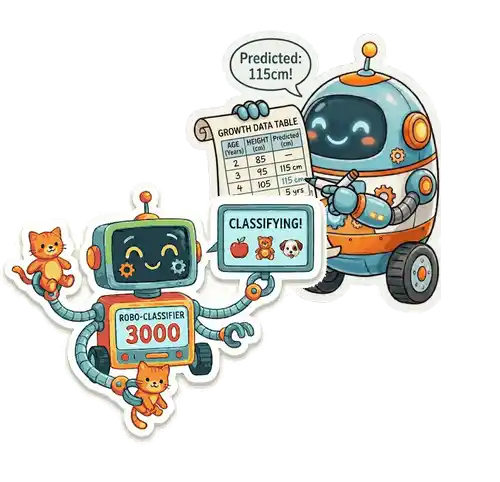
\includegraphics[height=3.8cm,keepaspectratio]{images/robots-prediction.png}\\[0.6em]
  \textbf{Prédiction}\\[0.2em]
  \textit{\small «~Étant donné une entrée, prédire une sortie~»}\\[0.2em]
  {\small Reconnaissance faciale, scores de crédit, etc.}
\end{minipage}%
\hfill
\begin{minipage}[b]{0.31\textwidth}
  \centering
  
\includegraphics[height=3.8cm,keepaspectratio]{images/robot-thumbsup.png}\\[0.6em]
  \textbf{Similarité}\\[0.2em]
  \textit{\small «~Étant donné une entrée, trouver des correspondances probables~»}\\[0.2em]
  {\small Spotify, applis de rencontre, etc.}
\end{minipage}%
\hfill
\begin{minipage}[b]{0.31\textwidth}
  \centering
  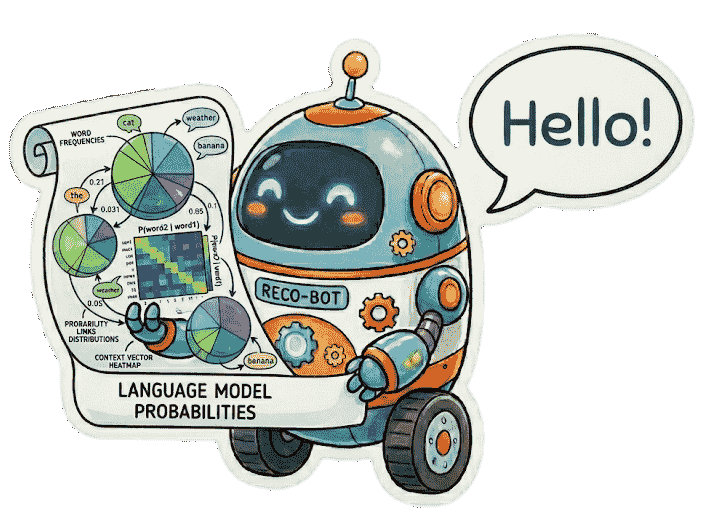
\includegraphics[height=3.8cm,keepaspectratio]{images/robot-statistics.png}\\[0.6em]
  \textbf{Génération}\\[0.2em]
  \textit{\small «~Invente une histoire — avec des images~! — à propos d'un éléphant~»}\\[0.2em]
  {\small ChatGPT, Stable Diffusion, Gemini, etc.}
\end{minipage}
\end{center}

Dans l'apprentissage automatique, l'ordinateur analyse beaucoup de données, puis identifie des motifs dans ces données en utilisant des statistiques. L'apprentissage automatique peut être appliqué à un ensemble incroyablement diversifié de données (texte, cartes, images, films, chansons, etc.), pour faire des prédictions, trouver des similarités, et même générer de nouvelles images, histoires, etc.

\begin{keypointbox}
  Alors que l'IA est souvent présentée comme quelque chose de «~magique~», l'apprentissage automatique est en réalité très concret~: \textbf{ce n'est qu'un ensemble d'algorithmes~!}
\end{keypointbox}

\begin{activitybox}
  Jouons avec de vrais outils qui utilisent l'IA, et voyons si nous pouvons comprendre comment ils pourraient fonctionner\ldots{}
\end{activitybox}

% ---------- Investigate : Modèles prédictifs ----------
\subsection{Exploration}

\subsubsection{Modèles prédictifs}

\img{images/robot-animals.png}{width=0.4\textwidth}{Un robot ramassant des peluches pour déterminer si ce sont des fruits, des chats ou des chiens}

Il existe plusieurs types de \textbf{modèles prédictifs} avec lesquels vous interagissez probablement tous les jours~!

\paragraph{Modèles de classification} — également appelés \textbf{classificateurs} — visent à \textbf{prédire des catégories}~:

\begin{itemize}
  \item Est-ce un courrier indésirable ou non~?
  \item Cette personne est-elle un enfant, un·e adolescent·e, ou un·e adulte~?
  \item Ce client est-il susceptible d'acheter un jeu vidéo ou non~?
  \item Dans quelle maison de Poudlard serais-je~?
\end{itemize}

\begin{activitybox}
  \textbf{Essayez un classificateur d'images~!}

  Le lien (Nyckel) vous mènera à un exemple d'outil d'apprentissage automatique qui prend une image de fleur et essaie de prédire à quelle \textbf{catégorie} de fleur elle appartient.

  \begin{itemize}
    \item Trouvez une image de fleur et glissez-la dans la boîte.
    \item Quelle(s) partie(s) de l'image pensez-vous que l'outil regarde pour faire sa prédiction~?
  \end{itemize}
\end{activitybox}

\begin{thinkbox}
  Réfléchissons un peu à la façon dont les classificateurs pourraient fonctionner~!

  Avec un·e partenaire, complétez la première section sur \textbf{Modèles Prédictifs~: Classificateurs}. Soyez prêts à partager~!
\end{thinkbox}

\begin{itemize}
  \item Le classificateur a-t-il bien identifié les fleurs~?
  \begin{itemize}
    \item Oui.
  \end{itemize}
  \item Qu'avez-vous remarqué sur les différences entre les deux images de fleurs~?
  \begin{itemize}
    \item Forme\ldots{} teinte\ldots{} bords lisses ou ondulés sur les pétales.
  \end{itemize}
  \item Comment pensez-vous que l'outil rapporte sa «~confiance~»~?
  \begin{itemize}
    \item Peut-être a-t-il une définition de la «~roséité~», et il calcule simplement à quelle distance la définition de \textbf{cette rose} se trouve de celle qu'il connaît.
  \end{itemize}
\end{itemize}

\begin{itemize}
  \item Vous venez d'examiner un problème de classification \emph{catégorielle}~: chaque image de fleur appartient à une catégorie de fleur.
  \item Parfois, un classificateur choisit simplement entre \textbf{deux} catégories~:
  \begin{itemize}
    \item «~Cet animal est-il un chien ou un chat~?~»
    \item «~Cette photo est-elle celle d'une personne jeune ou âgée~?~», etc.
  \end{itemize}
  \item Explorons un classificateur avec plus de deux sorties, en complétant la dernière section sur \textbf{Modèles Prédictifs~: Classificateurs}.
  \item Soyez prêts à partager~!
\end{itemize}

\begin{thinkbox}
  \begin{itemize}
    \item Quelles étaient vos prédictions pour chaque ligne~?
    \begin{itemize}
      \item Il n'y a pas de bonne réponse ici — l'important est de voir le degré d'accord ou de désaccord dans la classe.
    \end{itemize}
    \item Pourquoi n'avons-nous pas tous fait les mêmes prédictions~?
    \begin{itemize}
      \item Nous avons pris des décisions différentes sur les colonnes que nous valorisions le plus.
    \end{itemize}
    \item Quelle colonne était \textbf{la plus utile} pour classer les espèces~? Pourquoi~?
    \begin{itemize}
      \item \texttt{pattes} classe immédiatement les escargots (0), les tarentules (8) et tout le reste (4).
      \item \texttt{poids} classe immédiatement les chiens (généralement les plus lourds), les chats (généralement au milieu) et tout le reste (très léger).
    \end{itemize}
  \end{itemize}
\end{thinkbox}

\subsubsection{Modèles de régression}

\img{images/robots-prediction.png}{width=0.5\textwidth}{Un robot fait une prédiction sur un objet, un autre sur la taille future d'un enfant}

Mais les classificateurs ne sont pas le seul type de système de prédiction~!

Les classificateurs prédisent des \emph{catégories}. La \textbf{régression} prédit des \textbf{quantités}~:

\begin{itemize}
  \item Combien de paniers à trois points prédisons-nous pour un joueur qui mesure 1,95~m~?
  \item Combien de temps prédisons-nous qu'une personne vivra, sur la base d'un revenu de 95~000~\$~?
  \item Quelle est la probabilité qu'un·e étudiant·e réussisse à l'université, sur la base d'un score SAT de 1028~?
\end{itemize}

\begin{activitybox}
  \begin{itemize}
    \item Réfléchissons à la façon dont les modèles de régression pourraient fonctionner~!
    \item Avez-vous déjà passé un de ces quiz en ligne ridicules qui prétendent prédire combien de temps vous vivrez ou combien d'argent vous gagnerez sur la base de quelques questions~?
    \item Avec un·e partenaire, complétez la première section de \textbf{Modèles Prédictifs~: Régression}.
    \item Soyez prêts à partager~!
  \end{itemize}
\end{activitybox}

\begin{itemize}
  \item Quelles variables avez-vous trouvées~?
  \item Parmi vos pentes, y en avait-il des négatives~? Quel serait un exemple de pente négative~?
  \begin{itemize}
    \item Exemple~: nombre de paquets de cigarettes fumés par semaine.
  \end{itemize}
  \item Si toutes les variables sont à zéro, combien de temps votre quiz prédit-il qu'une personne vivra~?
  \begin{itemize}
    \item Pourquoi cela s'appelle-t-il l'ordonnée à l'origine~?
  \end{itemize}
\end{itemize}

Les humains essaient de trouver des formules pour nous aider à faire des prédictions sur tout, du moment où il pleuvra à la probabilité que vous remboursiez un prêt. Ces prédictions sont basées sur des \textbf{données}, plutôt que sur des suppositions comme «~les chats vous rendront plus riche~». Examinons des données réelles et essayons de faire une prédiction\ldots{}

\img{images/scatter-plot.png}{width=0.55\textwidth}{Nuage de points semaines-vs-poids avec un groupe serré en bas à gauche et quelques points vers la droite et le coin supérieur droit}

\begin{itemize}
  \item Qu'avez-vous remarqué sur le nuage de points~?
  \begin{itemize}
    \item Il semblait y avoir un motif.
    \item Certains points étaient vraiment loin des autres~!
    \item Beaucoup de points étaient regroupés à gauche.
  \end{itemize}
  \item Quel type de motif avez-vous vu~?
  \begin{itemize}
    \item Une ligne montant vers la droite.
  \end{itemize}
\end{itemize}

\begin{instructornotes}
  Si vous avez un projecteur et un tableau blanc, c'est le moment idéal pour faire dessiner aux élèves leurs différentes droites d'ajustement au tableau~!
\end{instructornotes}

Presque tout le monde a vu une ligne avec une pente positive, mais pas nécessairement la \emph{même} ligne exacte.

\begin{activitybox}
  Complétez la première section de \textbf{Modèles Prédictifs~: Régression}. Soyez prêts à partager~!
\end{activitybox}

\begin{itemize}
  \item Combien de temps avez-vous prédit qu'il faudrait pour que Daisy soit adoptée~? Et Maple~?
  \begin{itemize}
    \item Les réponses varieront.
  \end{itemize}
  \item Pourrions-nous écrire l'équation de cette droite~?
  \item Actuellement, nous traçons notre droite sur la base d'un nuage de points de tous les types d'animaux. Obtiendrions-nous un meilleur ajustement en regardant chaque espèce séparément~?
  \begin{itemize}
    \item Probablement~! Chaque espèce doit avoir un taux de croissance qui peut être représenté graphiquement, mais en les combinant toutes, on obtient une droite qui est un mélange de toutes les espèces différentes, et qui n'est bonne pour prédire aucune espèce en particulier.
  \end{itemize}
  \item Y a-t-il une autre colonne de nombres que nous pourrions utiliser pour prédire le temps d'adoption~?
  \begin{itemize}
    \item L'âge.
  \end{itemize}
\end{itemize}

\subsubsection{Modèles de similarité et de recommandation}

\img{images/robot-thumbsup.png}{width=0.35\textwidth}{Un robot tenant un livre avec un pouce levé sur la couverture}

Les \textbf{modèles de similarité et de recommandation} visent à \textbf{mesurer les différences}~:

\begin{itemize}
  \item Quelles chansons ressemblent le plus à celle-ci~?
  \item Quelles personnes sur un site de rencontre sont les meilleures correspondances pour cette personne~?
  \item Quelles dissertations sont les plus similaires à celle-ci~?
\end{itemize}

\begin{activitybox}
  \textbf{Démonstration Spotify~:}

  Recherchez une chanson que vos élèves reconnaîtront, en filtrant par «~chansons~». Survolez l'un des résultats de recherche et cliquez sur les trois points (\texttt{...}) qui apparaissent à droite. Sélectionnez «~Aller à la Radio de la chanson~».

  \begin{center}
    \textit{À quel point les recommandations de Spotify étaient-elles similaires à la chanson originale~?}
  \end{center}
\end{activitybox}

\begin{thinkbox}
  \begin{itemize}
    \item Réfléchissons à la façon dont les modèles de similarité pourraient fonctionner~!
    \item Avec un·e partenaire, complétez \textbf{Apprentissage par Similarité}.
    \item Soyez prêts à partager~!
  \end{itemize}
\end{thinkbox}

\begin{itemize}
  \item À votre avis, à quoi Spotify faisait-il attention lorsqu'il recommandait des chansons similaires à celle que nous avons choisie~?
  \begin{itemize}
    \item Les réponses varieront (volume, durée, tempo\ldots).
  \end{itemize}
  \item Quand vous téléchargez une image dans Google Recherche, à quoi prête-t-il attention pour recommander des images similaires~?
  \begin{itemize}
    \item Les réponses varieront (luminosité, couleur, symétrie\ldots).
  \end{itemize}
\end{itemize}

\subsubsection{Modèles génératifs}

\img{images/robot-statistics.png}{width=0.35\textwidth}{Un robot tenant une feuille avec des statistiques, avec une bulle disant «~Bonjour~»}

Les \textbf{modèles génératifs} recherchent des \textbf{motifs et des fréquences dans le langage}. On les appelle d'ailleurs souvent «~modèles de langage~» (\emph{language models})~:

\begin{itemize}
  \item Les ML entraînés sur \emph{l'anglais} peuvent être des «~agents conversationnels~» et générer des réponses en anglais.
  \item Les ML entraînés sur \emph{l'espagnol} peuvent être des «~agents conversationnels~» et générer des réponses en espagnol.
  \item Les ML entraînés sur \emph{la musique} peuvent être des «~robots musiciens~» et générer de la musique.
  \item Les ML entraînés sur \emph{les dessins} peuvent être des «~robots artistes~» et générer des images.
  \item Les ML entraînés sur \emph{le Morpion} peuvent être des «~robots de Morpion~» et générer des coups dans le jeu.
\end{itemize}

\begin{activitybox}
  Voici un exemple d'outil de ML sous forme d'agent conversationnel~: il génère du texte en réponse à ce que vous écrivez, en se basant sur des motifs qu'il a repérés en traitant des billions d'exemples.

  \begin{center}
    \textit{Donnez 1 à 2 minutes aux élèves pour essayer de discuter avec l'outil.}
  \end{center}
\end{activitybox}

\begin{instructornotes}
  Nous aborderons les modèles de langage dans une leçon ultérieure, mais pour l'instant l'important est de réaliser qu'il s'agit encore d'un autre type d'apprentissage automatique.
\end{instructornotes}

% ---------- Synthesize ----------
\subsection{Synthèse}

\begin{activitybox}
  Donnez aux élèves des exemples de cas d'usage et demandez-leur d'identifier le type de ML à l'œuvre.
\end{activitybox}

\newpage

% ===========================================================================
% SECTION 3 : QU'EST-CE QU'UN MODÈLE ?
% ===========================================================================
\section{Qu'est-ce qu'un modèle, au juste~?}

\begin{overviewbox}
  Les élèves commencent à réfléchir à la signification du terme «~modèle~», un terme large que différentes disciplines utilisent de manières subtilement différentes. L'objectif de cette section est de leur donner le début d'une intuition pour penser les modèles, \emph{pas} une définition rigoureuse~!
\end{overviewbox}

% ---------- Launch ----------
\subsection{Lancement}

Dans cette leçon, vous avez déjà vu le mot «~modèle~» utilisé en lien avec l'IA. Nous avons parlé de \textbf{modèles de prédiction} comme les modèles de classification et les modèles de régression. Nous avons parlé de \textbf{modèles génératifs} (de langage), et vous en connaissez probablement certains célèbres comme GPT, Gemini, ou Claude.

\begin{thinkbox}
  \centering
  \textbf{Mais qu'est-ce qu'un MODÈLE, au juste~?}
\end{thinkbox}

\begin{keypointbox}
  \textbf{Un modèle est un résumé mathématique d'un jeu de données.}
\end{keypointbox}

Définir le terme «~modèle~» est en réalité assez difficile, car différentes disciplines définiraient le même mot de manières légèrement différentes~! Mais ce qu'elles ont toutes en commun, c'est que les modèles sont utilisés pour \emph{représenter un jeu de données}, et ce de manière plus compacte. Quand nous résumons une dissertation, nous essayons d'\textbf{identifier les idées principales} et de \textbf{laisser le reste de côté} — les modèles font la même chose avec les données, en identifiant les motifs ou structures les plus importants et en laissant le reste de côté.

\begin{center}
  \fbox{%
    \begin{minipage}{0.85\textwidth}
      \centering
      \textbf{Tous les modèles résument les caractéristiques d'un jeu de données,}\\
      \textbf{et tous les modèles laissent certains détails de côté~!}
    \end{minipage}%
  }
\end{center}

Vous connaissez peut-être déjà certains modèles mathématiques simples~:

\begin{itemize}
  \item La \textbf{moyenne}, la \textbf{médiane} et le \textbf{mode} sont différentes façons de résumer le «~centre~» d'une liste de nombres, mais ils laissent de côté la liste originale.
  \item Une \textbf{droite d'ajustement} (\emph{line of best fit}) résume la relation entre les points d'un nuage de points, mais elle laisse de côté les points originaux.
\end{itemize}

Ces deux exemples nous disent quelque chose sur une caractéristique du jeu de données original, et laissent de côté les détails moins importants.

\begin{instructornotes}
  \textbf{Toutes les définitions ne sont pas binaires~!}

  Une personne issue du milieu de l'apprentissage automatique dirait que la moyenne d'une liste de nombres n'est pas du tout un modèle~! En apprentissage automatique, les modèles sont généralement utilisés pour \emph{faire des prédictions}. Un·e mathématicien·ne ne serait pas d'accord.

  Le fait est que ces lignes sont quelque peu floues, et pour un cours d'introduction nous avons essayé d'adopter une approche de plus petit dénominateur commun en nous concentrant sur deux idées principales communes à toutes les disciplines~: \textbf{(a)} les modèles résument les caractéristiques d'un jeu de données, et \textbf{(b)} ce résumé laisse de côté des parties du jeu de données.
\end{instructornotes}

% ---------- Investigate ----------
\subsection{Exploration}

\begin{center}
  \fbox{%
    \begin{minipage}{0.8\textwidth}
      \centering
      \textit{«~Tous les modèles sont faux. Certains sont utiles.~»}
    \end{minipage}%
  }
\end{center}

Par définition, un modèle laisse de côté certains détails du jeu de données original.

\begin{itemize}
  \item Les heures de pointe se situent généralement entre 16h30 et 18h30 (mais pas les week-ends fériés~!)
  \item Le blanc est la couleur de voiture la plus répandue dans le monde (mais des millions de voitures ne sont pas blanches~!)
\end{itemize}

\begin{keypointbox}
  Le but d'un modèle n'est pas d'avoir raison à chaque fois, mais d'être \emph{suffisamment juste pour être utile}. Les deux généralisations ci-dessus sont parfois fausses. Mais si vous planifiez un voyage en voiture, une seule est utile.
\end{keypointbox}

\begin{activitybox}
  \begin{itemize}
    \item Pouvez-vous trouver votre propre exemple de modèle~?
    \begin{itemize}
      \item Quelques idées~:
      \begin{itemize}
        \item Une courbe de taille, de poids ou d'IMC chez le médecin (un résumé de la croissance d'une population).
        \item Les prévisions météorologiques (un résumé des tendances et relations environnementales).
      \end{itemize}
    \end{itemize}
    \item Quand votre modèle est-il faux~?
    \begin{itemize}
      \item Un bodybuilder a un IMC dangereusement élevé, mais il n'est pas réellement en mauvaise santé.
      \item Les bulletins météo peuvent mal évaluer la température ou la probabilité de pluie.
    \end{itemize}
    \item Votre modèle est-il utile~?
    \begin{itemize}
      \item Les réponses varieront.
    \end{itemize}
  \end{itemize}
\end{activitybox}

% ---------- Synthesize ----------
\subsection{Synthèse}

\begin{center}
  \fbox{%
    \begin{minipage}{0.85\textwidth}
      \centering
      \textbf{Les modèles résument les caractéristiques d'un jeu de données,}\\
      \textbf{et laissent les détails de côté.}
    \end{minipage}%
  }
\end{center}

\begin{thinkbox}
  \begin{itemize}
    \item Quelles caractéristiques pensez-vous que notre classificateur de fleurs examinait lorsqu'il comparait une image à différentes espèces de fleurs~? Qu'est-ce qu'il ignorait~?
    \item Quelles caractéristiques pensez-vous que Spotify examine lorsqu'il compare des chansons~? Qu'est-ce qu'il ignore~?
    \item Quelles caractéristiques avez-VOUS regardées pour prédire le temps d'adoption des animaux dans notre refuge~? Qu'avez-vous ignoré~?
  \end{itemize}
\end{thinkbox}

\newpage

% ===========================================================================
% ANNEXE : INFORMATIONS DE LICENCE
% ===========================================================================
\section*{À propos de ces supports}

Ces supports ont été développés en partie grâce au soutien de la \emph{National Science Foundation} (bourses 1042210, 1535276, 1648684, 1738598, 2031479 et 1501927).

\begin{center}
  
\includegraphics[width=2cm]{images/CCbadge.png}

  \textbf{Bootstrap} par la Communauté Bootstrap est sous licence Creative Commons 4.0 Unported.\\
  Cette licence n'accorde pas la permission d'organiser des formations ou du développement professionnel.\\
  Offrir des formations ou du développement professionnel avec des supports substantiellement dérivés de Bootstrap\\
  doit être approuvé par écrit par un directeur de Bootstrap.\\
  Les autorisations au-delà du cadre de cette licence, telles que l'organisation de formations,\\
  peuvent être disponibles en contactant \href{mailto:contact@bootstrapworld.org}{contact@bootstrapworld.org}.
\end{center}

\vspace{1cm}

\begin{center}
  \textit{Traduction française réalisée le 15 juillet 2026.}\\
  \textit{Source originale~: \url{https://www.bootstrapworld.org/materials/fall2026/en-us/lessons/ai-intro/index.shtml?pathway=ai}}
\end{center}

% ===========================================================================
% TABLE DES ILLUSTRATIONS
% ===========================================================================
\newpage
\section*{Liste des illustrations}

Les images suivantes sont incluses dans le dossier \texttt{images/}~:

\begin{enumerate}[leftmargin=*]
  \item \texttt{algorithme-flowchart.png} — Organigramme d'un algorithme générique
  \item \texttt{john-mccarthy.png} — Portrait de John McCarthy
  \item \texttt{robots-prediction.png} — Robots illustrant la prédiction
  \item \texttt{robot-thumbsup.png} — Robot avec un pouce levé (similarité)
  \item \texttt{robot-statistics.png} — Robot avec des statistiques (génération)
  \item \texttt{robot-animals.png} — Robot triant des peluches (classification)
  \item \texttt{scatter-plot.png} — Nuage de points semaines-vs-poids
  \item \texttt{CCbadge.png} — Badge Creative Commons
\end{enumerate}

\vspace{1em}
\textbf{Source originale~:} \url{https://www.bootstrapworld.org/materials/fall2026/en-us/lessons/ai-intro/index.shtml?pathway=ai}

\end{document}
